\documentclass[12pt]{article}
\usepackage{fullpage}
\usepackage{enumerate}
\usepackage{multicol}
\usepackage{comment}
\usepackage{lastpage}
\usepackage{fancyhdr}
\pagestyle{fancy}

\addtolength{\topmargin}{-0.25in}
\usepackage{graphicx,tikz}
\usepackage{tkz-euclide}
\usetkzobj{all}	
\usepackage{array, multicol}
\usepackage{amsmath}

\everymath{\displaystyle}

\fancypagestyle{plain}{
	\fancyhf{}
	\addtolength{\headheight}{2.92\baselineskip}
	\lhead{\bf MATH 2574 (Calculus III) \\
		Fall 2015 \\
		}
	\rhead{{\large \bf SOLUTIONS}%{Name:} \underline{\hspace{40ex}} 
		\\
		\vspace{0.5pc}
		Tues 15 Sep 2015}
	\rfoot{Quiz 3 {\bf SOLS} p.\thepage\ (of \pageref{LastPage})}
	}
\fancyhf{}
\renewcommand{\headrulewidth}{0pt}

\title{\flushleft\vspace{-1.5pc}\Large
	\bf Quiz 3: Trajectories and Arc Length ($\textstyle\oint$11.7-11.8)}
\author{}
\date{}

\rfoot{Quiz 3 {\bf SOLS} p.\thepage\ (of \pageref{LastPage})}

% % % % %
\begin{document}
\maketitle

\vspace{-5pc}
\noindent{\small \it Note: The typo in the course number as well as the typo in the half-angle formula have been fixed.}

\vspace{1pc}
\noindent{\bf Directions:} You have 30 minutes to complete this quiz.  You may collaborate.  

\vspace{1pc}
\begin{enumerate}[1.]
%\item {\bf (2 pts)} Find the length of the spiral $\rho(\theta)=e^{-a\theta}$ for $\theta\geq 0$, $a>0$.
\item {\bf (2 pts)} A cycloid is the path traced by a point on a rolling circle (think of a light on the rim of a moving bicycle wheel).  The cycloid generated by a circle of radius $a$ is given by the parametric equation 
\[
x=a(t-\sin{t}) \quad y=a(1-\cos{t}).
\]
\begin{enumerate}[(a)]
\item The parameter range $0\leq t\leq 2\pi$ produces one arch of the cycloid.  Compute its length.  {\bf Hint:} You might need the half-angle formula
\[
\sin^2{\theta}=\textstyle\frac{1}{2}\left(1-\cos{2\theta}\right).
\]

\vspace{1pc}
\noindent {\bf\underline{Solution}:} The length of the arch is given by the arc length formula; substitute the given values in the problem and simplify:
\[\begin{split}
\text{length of arch} &= \int_{0}^{2\pi}\sqrt{x'(t)^2+y'(t)^2}\ dt \\
	&= \int_{0}^{2\pi}\sqrt{\left(a(1-\cos{t})\right)^2+(a\sin{t})^2}\ dt \\
	&= \int_{0}^{2\pi}\sqrt{a^2\left(1-2\cos{t}+\cos^2{t}\right)+a^2\sin^2{t}}\ dt \\
	&= a\int_{0}^{2\pi}\sqrt{2-2\cos{t}}\ dt.
\end{split}\]
To evaluate the integral, first use the given half-angle formula,
\[\begin{split}
\sin^2{\theta} &= \textstyle\frac{1}{2}\left(1-\cos{2\theta}\right) \\
2\sin^2{\theta} &= 1-\cos{2\theta} \\
4\sin^2{\theta} &= 2-2\cos{2\theta} \\
4\sin^2{\left(\textstyle\frac{t}{2}\right)} &= 2-2\cos{t}, 
\end{split}\] 
having set $t=2\theta$.  Then the length of one arch is
\[\begin{split}
a\int_{0}^{2\pi}\sqrt{2-2\cos{t}}\ dt &= a\int_{0}^{2\pi}\sqrt{4\sin^2{(\textstyle\frac{t}{2})}}\ dt \\
	&= a\int_{0}^{2\pi}2\sin{\left(\textstyle\frac{t}{2}\right)}\ dt \\
	&= a\left(\left.-4\cos{\left(\textstyle\frac{t}{2}\right)}\right\vert_{0}^{2\pi}\right) \\
	&= a\left[-4\cos{\pi}-(-4\cos{0})\right] \\
	&= a\left[-4(-1)-(-4)\right] \\
	&\boxed{= 8a.}
\end{split}\]
\vspace{2pc}
\item Draw a well-labelled graph of the arch of the cycloid.

\vspace{1pc}
\noindent {\bf\underline{Solution}:} In order to draw the graph without a calculator, use techniques from Cal I (see $\textstyle\oint$4.3 in the text for more information).

\vspace{1pc}
First examine the derivatives.  For the entire domain $0\leq t\leq 2\pi$, 
\[
x'(t)=a(1-\cos{t})\geq 0,
\]
i.e., $x(t)$ increases as $t$ increases.  This means the graph will be drawn from left to right.  Furthermore, $x'(t)$ is symmetric about the point $t=\pi$ so the rate at which the $x$-coordinate is drawn will also be symmetric about $x(\pi)=a\pi$.  Similarly, the $y$-coordinate has derivative
\[
y'(t)=a\sin{t},
\]
which is antisymmetric about the point $t=\pi$, so the $y$-coordinate increases for $0< t< \pi$ and decreases $\pi < t < 2\pi$.  Its maximum value is $y(\pi)=2a$.

\vspace{1pc}
Now examine the derivative of $y$ as a function of $x$:
\[\begin{split}
\frac{dy}{dx} &= \frac{y'(t)}{x'(t)} = \frac{a\sin{t}}{a(1-\cos{t})}
\end{split}\]
(The factor $a$ in both the numerator and denominator can be disregarded.)  Considering the given domain $0\leq t\leq 2\pi$, the derivative is undefined for $t=0,2\pi$ and zero for $t=\pi$.  From the information above about $x'(t)$ and $y'(t)$, the derivative $\textstyle\frac{dy}{dx}$ is positive for $0 < t <\pi$ (so $y$ is increasing as a function of $x$) and negative for $\pi < t < 2\pi$ (so $y$ is decreasing as a function of $x$).  The second derivative,
\[\begin{split}
\frac{d^2y}{dx^2} &= \frac{d}{dx}\left(\frac{\sin{t}}{1-\cos{t}}\right) \\
	&= \frac{\frac{d}{dt}\left(\frac{\sin{t}}{1-\cos{t}}\right)}{\frac{dx}{dt}} \\
	&= \frac{\frac{(1-\cos{t})(\cos{t})-\sin{t}(\sin{t})}{\left(1-\cos{t}\right)^2}}{a(1-\cos{t})} \\
	&= \frac{\cos{t}-(\cos^2{t}+\sin^2{t})}{a(1-\cos{t})^3} \\
	&= \frac{-(1-\cos{t})}{a(1-\cos{t})^3} \\
	&= \frac{-1}{a(1-\cos{t})^2}, 
\end{split}\]
is always negative, so the graph will be concave down.

\vspace{1pc}
Finally, compute some key coordinates $(x(t),y(t))$, using values in the domain $0\leq t\leq 2\pi$: 
\begin{alignat*}{4}
x(0) &= a(0-\sin{0})=0 &\qquad y(0) &= a(1-\cos{0})=0 \\
x(2\pi) &= a(2\pi-\sin{2\pi})=2a\pi &\qquad y(2\pi) &=a(1-\cos{2\pi})=0
\end{alignat*}
\includegraphics[scale=0.83]{Q3pic}
\end{enumerate}

\newpage
\item A golf ball has an initial position 
\[
\overrightarrow{r}(0)=\langle x_0,y_0\rangle = \langle 0,0\rangle = 0\hat i + 0\hat j \text{ ft}
\]
when it is hit at an angle of $30^{\circ}$ from the ground and with an initial speed of $150$ ft/s.  For the following, neglect air resistance and assume gravity is a constant $g=32$ ft/s$^2$.  {\bf You must include units in your answers to receive credit.}
	\begin{enumerate}[(a)]
	\item {\bf (1 pt)} The golf ball's acceleration vector is: $\overrightarrow{a}(t)=$
	
	\vspace{0.5pc}
	{\bf\underline{Solution}.} $\boxed{\langle 0,-32\rangle\text{ ft/s$^2$}}$, %\newline
	because there is no air resistance, and the only other force on the ball given is gravity, which is negative, according to the given coordinate system.
	
	\vspace{1pc} 
	\item {\bf (1 pt)} Its initial speed is: $|\overrightarrow{v}(0)|=$
	
	\vspace{0.5pc}
	{\bf\underline{Solution}.} $\boxed{150\text{ ft/s}}$ (it was given in the problem).
	
	\vspace{1pc}
	\item {\bf (1 pt)} Its initial velocity is: $\overrightarrow{v}(0)=$
	
	\vspace{0.5pc}
	{\bf\underline{Solution}.} $\boxed{\langle 75\sqrt{3},75\rangle\text{ ft/s.}}$  To see why, use the initial angle of the golf ball's trajectory.  The initial speed is the hypotenuse of a special triangle:  
	\begin{center}
	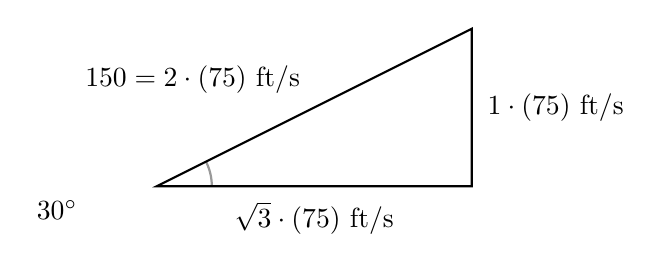
\begin{tikzpicture}[thick]
	\coordinate (O) at (0,0);
	\coordinate (A) at (-4,0);
	\coordinate (B) at (0,2);
	\draw (O)--(A)--(B)--cycle;
	\tkzLabelSegment[below=2pt](O,A){$\sqrt{3}\cdot(75)\text{ ft/s}$}
	\tkzLabelSegment[right=2pt](O,B){$1\cdot(75)\text{ ft/s}$}
	\tkzLabelSegment[above left=2pt](A,B){$150=2\cdot(75)\text{ ft/s}$}
	\tkzMarkAngle[size=0.7cm,opacity=.4](O,A,B)
	\tkzLabelAngle[pos = 1.3](B,A,O){$30^{\circ}$}
	\end{tikzpicture}
	\end{center}
	The base of the triangle is in the $\hat i$-direction and the height of the triangle is in the $\hat j$-direction.
	
	\vspace{1pc}
	\item {\bf (1 pt)} The golf ball's velocity vector is $\overrightarrow{v}(t)=$
	
	\vspace{0.5pc}
	{\bf\underline{Solution}.} $\boxed{\langle 75\sqrt{3},75-32t\rangle\text{ ft/s}.}$  The velocity vector is one of the solutions of the indefinite integral
	\[
	\int \overrightarrow{a}(t)\ dt = \int \langle 0,-32\rangle\ dt = \langle 0,-32t\rangle + \overrightarrow{C}.
	\]
	The initial value computed in (c) gives the correct constant vector $\overrightarrow{C}$:
	\[
	\overrightarrow{v}(0)=\langle 0,-32\cdot(0)\rangle + \overrightarrow{C} = \langle 75\sqrt{3},75\rangle 
	\]
		
	\vspace{1pc}
	\item {\bf (1 pt)} The golf ball's position vector is $\overrightarrow{r}(t)=$
	
	\vspace{0.5pc}
	{\bf\underline{Solution}.} $\boxed{\langle 75\sqrt{3}t,75t-16t^2\rangle\text{ ft}}$ is found using the same procedure as in (d):
	\[\begin{split}
	\int \overrightarrow{v}(t)\ dt &= \int \langle 75\sqrt{3},75-32t\rangle\ dt = \langle 75\sqrt{3}t,75t-32\left(\textstyle\frac{1}{2}t^2\right)\rangle + \overrightarrow{C} \\
	\overrightarrow{r}(0) &= \langle 75\sqrt{3}\cdot(0),75\cdot(0)-32\left(\textstyle\frac{1}{2}\cdot(0)^2\right)\rangle + \overrightarrow{C} =\langle x_0,y_0\rangle = \langle 0,0\rangle
	\end{split}\]
	
	\vspace{1pc}
	\item {\bf (1 pt)} Determine the golf ball's time of flight.
	
	\vspace{0.5pc}
	{\bf\underline{Solution}.} The vertical component of the golf ball's trajectory is given by a parabola $y(t)=75t-16t^2$ whose zeros are exactly when the golf ball hits the ground.  
	\[\begin{split}
	y(t)=0 &= 75t-16t^2 \\
		&= t(75-16t) \\
	\implies & t=0,\textstyle\frac{75}{16}
	\end{split}\]
	The solution $t=0$ is when the golf ball is hit.  The next time the ball is on the ground is after $\boxed{t=\textstyle\frac{75}{16}\text{ s.}}$
	
	\vspace{1pc}
	\item {\bf (1 pt)} How far does the golf ball travel?
	
	\vspace{0.5pc}
	{\bf\underline{Solution}.} The distance is exactly the $x$-component of the position vector, evaluated at the time from (f):
	\[\begin{split}
	x(t) &= 75\sqrt{3}t \\
	x\left(\textstyle\frac{75}{16}\right) &= 75\sqrt{3}\cdot\left(\textstyle\frac{75}{16}\right) \\
		&\boxed{= \textstyle\frac{75^2\sqrt{3}}{16}\text{ ft.}}
	\end{split}\]
	
	\vspace{1pc}
	\item {\bf (1 pt)} What is the maximum height of the golf ball? 
	
	\vspace{0.5pc}
	{\bf\underline{Solution}.} The maximum height is the vertex of the parabola in the $y$-component of $\overrightarrow{r}(t)$.  There are several ways to compute it, one is to evaluate at the zero of the derivative:
	\[\begin{split}
	y'(t)=0 &= 75-32t \\
	\implies & t=\textstyle\frac{75}{32}
	\end{split}\]
	is when $y(t)$ attains its maximum; 
	\[
	y\left(\textstyle\frac{75}{32}\right) = 75\cdot\left(\textstyle\frac{75}{32}\right) + 16\cdot\left(\textstyle\frac{75}{32}\right)^2 = \textstyle\frac{75^2}{32}-\textstyle\frac{1}{2}\left(\frac{75^2}{32}\right) = \textstyle\frac{1}{2}\left(\frac{75^2}{32}\right) \boxed{= \textstyle\frac{75^2}{64}\text{ ft.}} 
	\]
	
	\end{enumerate}
\end{enumerate}
% % % % %
\end{document}